\begin{figure}[h]
    \centering
    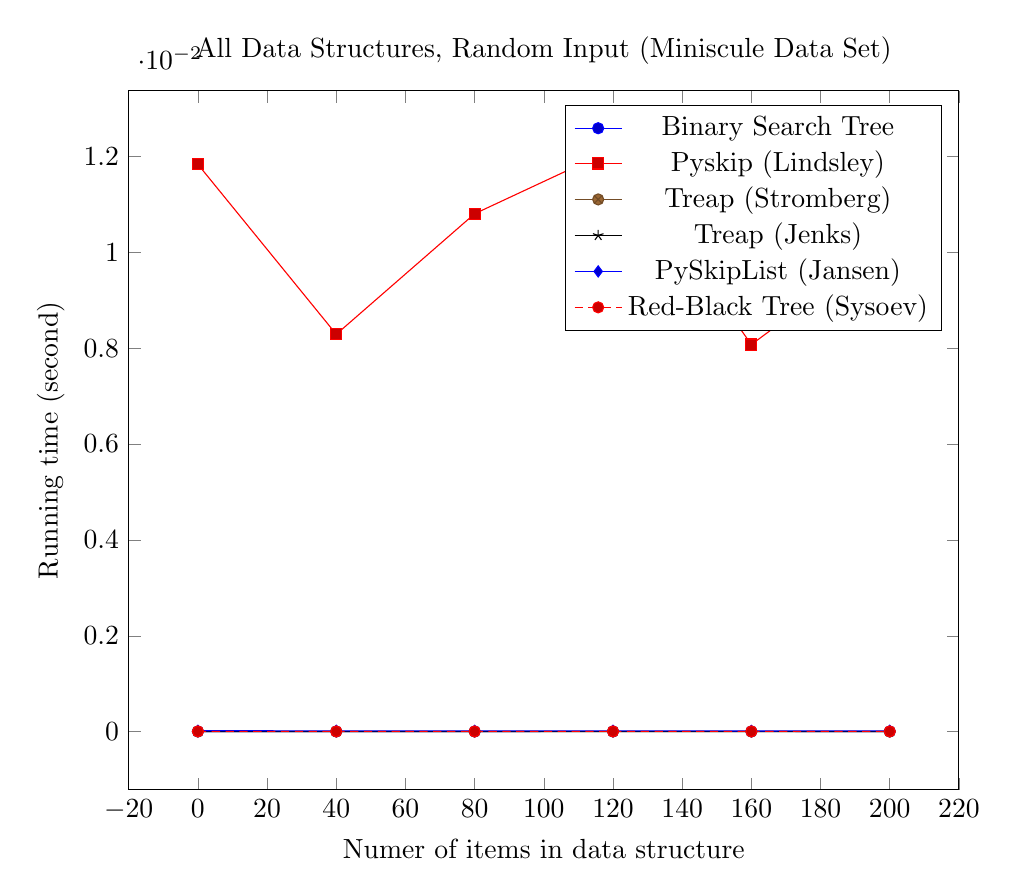
\begin{tikzpicture}
        \begin{axis}[
            xlabel={Numer of items in data structure},
            ylabel={Running time (second)},
            title={All Data Structures, Random Input (Miniscule Data Set)},
            width=\textwidth
        ]
		\addplot coordinates {
			(0, 6.17409440337724e-06)
			(40, 6.143976869665835e-06)
			(80, 6.324682071934263e-06)
			(120, 6.505387273847419e-06)
			(160, 6.535504807558823e-06)
			(200, 6.14397686984347e-06)
		};
		\addplot coordinates {
			(0, 0.011833690979045741)
			(40, 0.008289248793416349)
			(80, 0.010803099094215262)
			(120, 0.012149322731961476)
			(160, 0.008075384186789058)
			(200, 0.01021707212396361)
		};
		\addplot coordinates {
			(0, 5.451273595191708e-06)
			(40, 5.993389201286447e-06)
			(80, 5.029628123764951e-06)
			(120, 6.113859336132066e-06)
			(160, 5.08986319118776e-06)
			(200, 4.51763005120398e-06)
		};
		\addplot coordinates {
			(0, 2.8310481653193164e-06)
			(40, 2.2889325594022126e-06)
			(80, 2.108227357133785e-06)
			(120, 2.3190500931136173e-06)
			(160, 2.108227357133785e-06)
			(200, 2.1383448910228252e-06)
		};
		\addplot coordinates {
			(0, 2.0690745634865947e-05)
			(40, 1.909451634993786e-05)
			(80, 1.6865818858136095e-05)
			(120, 1.927522155220629e-05)
			(160, 1.6263468184618546e-05)
			(200, 1.9335456619451462e-05)
		};
		\addplot coordinates {
			(0, 7.95102889021848e-06)
			(40, 6.987267812519349e-06)
			(80, 6.746327543183383e-06)
			(120, 7.047502879942158e-06)
			(160, 6.927032745274176e-06)
			(200, 7.047502879942158e-06)
		};
        \legend{Binary Search Tree, Pyskip (Lindsley), Treap (Stromberg), Treap (Jenks), PySkipList (Jansen), Red-Black Tree (Sysoev)}
        \end{axis}
    \end{tikzpicture}
    \caption{Average of 10 operations, benchmarked every 40, starting at 0.}
\end{figure}